%

%% main.tex
%% V1.4b
%% 2015/08/26
%% by Michael Shell

\documentclass[journal]{IEEEtran}
\usepackage{enumerate}
\usepackage{algorithm}
\usepackage{algpseudocode}
\usepackage{subfigure}
\usepackage{pgfgantt}
\usepackage{url,xspace}
\usepackage{color,soul}
\newcommand{\tinyskip}{\vspace{2pt}}
\newcommand{\mypar}[1]{\tinyskip\noindent\textbf{#1.}\xspace}
% correct bad hyphenation here
%\hyphenation{op-tical net-works semi-conduc-tor}

\usepackage{changes}
\usepackage{color}

\begin{document}

\title{Throughput And Lifetime Maximisation For IoT Deployments In Unlicensed Spectral Bands}

\author{Noradila Nordin,
        Richard G Clegg,
        Yiannis Andreopoulos,
        and Miguel Rio% <-this % stops a space
\thanks{N. Nordin is with the School of Computing, University Utara Malaysia, Kedah, 06010, Malaysia (e-mail: nnoradila@uum.edu.my).}
\thanks{R. G. Clegg is with the School of Electronic Engineering and Computer Science, Queen Mary University, London, E1 4NS, UK (e-mail: richard@richardclegg.org).}% <-this % stops a space
\thanks{Y. Andreopoulos and M. Rio are with the Department
of Electronic \& Electrical Engineering, University College London, London,
WC1E 7JE, UK (e-mail: i.andreopoulos@ucl.ac.uk; miguel.rio@ucl.ac.uk).}% <-this % stops a space
%\thanks{Manuscript received April 19, 2005; revised August 26, 2015.}
}


% The paper headers
%%\markboth{Journal of \LaTeX\ Class Files,~Vol.~14, No.~8, August~2015}%
%%{Nordin \MakeLowercase{\textit{et al.}}: Maximising Throughput and Energy Lifetime in Wireless Sensor Networks}

% make the title area
\maketitle

% As a general rule, do not put math, special symbols or citations
% in the abstract or keywords.

\begin{abstract}
Internet-of-Things oriented data gathering  can be abstracted as wireless sensor networks (WSNs) that upstream measurements to aggregators in order to link to internet resources for analysis and reaction capabilities that surpass the aptitude of local processing. Within this context, the WSN part typically comprises an ad-hoc  deployment in a number of unlicensed spectral bands (channels) with unpredictable interference characteristics.  This results in frequent packet retransmissions  and high energy drain.
This paper presents a two-step technique to optimise such IoT deployments in terms of the throughput and WSN operational lifetime. 
The proposed multichannel cross-layer routing protocol (MCRP) detects excessive interference at the medium access control (MAC) layer and switches away from channels that experience excessive interference using a graph colouring approach. In order to prolong network lifetime, MCRP also incorporates a tree reconfiguration algorithm to find network topologies that use alternative routes based on the sensors' current energy status. 
Experimental results demonstrate that MCRP can achieve 80\% to 90\% of the throughput of the ideal (i.e., interference-free) MAC layer. In addition, simulated tests on large topologies show that MCRP  allows for more than eight-fold improvement in the WSN's lifetime.
\end{abstract}


% Note that keywords are not normally used for peerreview papers.
\begin{IEEEkeywords}
wireless sensor networks, Internet of Things, network lifetime, energy efficiency
\end{IEEEkeywords}

\IEEEpeerreviewmaketitle


\section{Introduction}

\IEEEPARstart{W}{ireless} sensor networks (WSNs) are widely used to gather data and measurement \added{from the physical world in order to enable advanced monitoring and control of engineered or physical infrastructures \cite{wsnsurvey}. In the last few years, a concerted effort has begun to make WSNs "internet-enabled", in order to allow for advanced monitoring or reaction capabilities that cannot be achieved by local processing alone. Within this Internet-of-Things (IoT) paradigm,}  it is increasingly important to have reliable and energy-efficient WSNs that could function for years, as sensors are often deployed in areas that are difficult to reach, such as volcanic monitoring \cite{volcano}, forest fire detection \cite{forestFire} and monitoring of dam structural integrity \cite{dam}.

However, \added{sensors have limited energy resources} as they are battery powered, and will not able to function once a certain threshold of energy level is reached. 
\added{IoT-oriented WSNs also operate in unlicensed bands, such as the 16 channels of the 2.400-2.484 GHz band \cite{80215} or the 7 channels of the 5.850-5.925 GHz band \cite{80211}, where interference from the unreliable radio environment} drains the sensors' batteries at a higher rate. These constraints have a major impact on the \added{WSN's throughput and lifetime characteristics. In order to cope with these limitations, one}  should be able to \added{adaptively  switch to reliable channels in order to reduce the effect of interference in the throughput and and energy drain of each sensor, and thereby maximise the} overall network lifetime.
Many energy-efficient \added{medium access control (MAC) or routing protocols have been proposed \cite{micmac, orchestra} \cite{winter2012rpl, ctp, leach}, with simulations showing promising results in advancing either throughput or energy autonomy, but very few joint MAC\ \&\ routing protocol in a single half-duplex radio interface \cite{chrysso, cmac, cognitiveSurvey} for throughput and lifetime maximisation have been experimentally tested in unlicensed bands yet}. %\textcolor{red}{SEE\ NOTE\ 1 - not in single radio, half duplex, need explanation}.

Multichannel cross-layer routing protocol (MCRP) is a new protocol that considers all available \added{channels in the unlicensed spectrum}. The protocol is partly distributed: nodes work independently, but strategic decisions are made by a centralised controller known as the low power border router (LPBR), \added{which is also the WSN aggregator that communicates with internet resources within an IoT-oriented deployment}. MCRP increases throughput by using the channels that are found to have the lowest interference for communications.
Energy-based tree reconfiguration is \added{then} used to improve network lifetime.  We show that MCRP is able to achieve 80\%-90\% of the optimal \added{(i.e., interference-free)} throughput in real world experiments.
MCRP also improves the energy efficiency consuming three times less energy than a single channel protocol.  It allows reconfiguration of topologies to increase the network lifetime, as measured by time to first node failure.  In simulation experiments, the time to first node failure was increased by a factor of 8.3 \added{in comparison to the no-reconfiguration case}.

An initial version of MCRP was introduced \added{in our related conference paper} \cite{mcrp}, which presented some basic emulation results for loss rates on a small network and a comparison with the single channel routing protocol for low-power and lossy networks (RPL) \cite{winter2012rpl}.  This paper extends the MCRP protocol to improve recovery and to allow topology reconfiguration.  It presents more extensive emulation results as well as real world implementation on hardware with a ten node network and simulation results on a several hundred node network.  The results are compared with another multi-channel protocol, Orchestra \cite{orchestra}, \added{which represents the state-of-the-art}.

This paper is organised as follows. Section \ref{RelatedWork} presents  related work, Section \ref{MCRP} explains the multichannel cross-layer routing protocol, the improvements in comparison to a single and existing multichannel protocols and evaluates MCRP performance in emulation and real world environments.
Section \ref{OptimalTree} describes the proposed energy-based tree reconfiguration for WSNs in detail.  Section \ref{MCRPemulation} tests MCRP in emulation and Section \ref{MCRPhardware} tests it in hardware.
Section \ref{PerformanceEvaluation} evaluates the performance of the proposed optimisation. Finally, Section \ref{Conclusion} concludes this paper.

\section{Related Work}
\label{RelatedWork}

\mypar{Network Lifetime} A major aim of MCRP is to increase network lifetime by optimising energy use. Various definitions of network lifetime are used in the literature, for example, Hellman et al. \cite{hellmanLifetime} and Xu et. al. \cite{gafLifetime} defined the network lifetime as the fraction of surviving nodes in the network, while Tian and Georganas \cite{tian2002coverage} measured the time until all nodes have been drained of their energy.
%for example the mean life time of all nodes \added{[r]}. 
In this paper we use the common definition of the time until the first node runs out of energy \cite{maxmin, erapl, lifetimedef1}.  Typically in networks with a central node providing upload to the network (LBPR) nodes closer to this in the topology carry more traffic and use more energy.  Energy use also increases in the presence of interference since packets may need to be transmitted multiple times to get a successful transmission. Two main ways to extend network lifetime are (i) multichannel MAC protocol to reduce multiple transmission due to interference and (ii) reconfiguring topologies to make less demand on nodes with low energy.

\mypar{Multichannel MAC Protocols}
Existing multichannel MAC protocols can be categorised into synchronous and asynchronous. Synchronous systems require tight time synchronisation to schedule communications and avoid collisions. Asynchronous systems self-configure but avoid the costs of synchronisation.
Channel hopping enables the packet to be communicated on a different frequencies to work around interference.  Orchestra \cite{orchestra} is a synchronous protocol that is based on the Time Slotted Channel Hopping (TSCH) \cite{tsch}. It uses channel hopping to increase the reliability in the network.  MiCMAC \cite{micmac} is an asynchronous MAC protocol that uses a distributed channel hopping protocol and switches to a different channel each time it wakes up.  Orchestra and MiCMAC use predefined hopping sequences in the hope of routing around channels with interference.  They use a limited subset of channels known to have low interference in typical settings. Previous work by Sha et al. \cite{homearea} and Mohammad et al. \cite{oppcast} found that the channel reliability changes over time in non cyclic manner, thus no specific channels could achieve a long term reliability. Stabellini \cite{energyluca} proposed a spectrum sensing algorithm to decide on the number of channels to be sensed before the channel is selected for transmissions.  By contrast to these approaches MCRP attempts to detect which channels have interference during operation and avoid them as the nodes connect.

\mypar{Routing Protocols}  
A major issue in WSN routing protocols is finding and maintaining energy efficient routes.  Topologies may need to change rapidly to avoid network disconnection due to interference.  However, topology changes can be costly in terms of messaging and packet loss.  RPL is a routing protocol that builds the topology based on an objective function related to link quality.  New metrics and constraints can be defined for RPL and this leads to several studies combining energy based metrics into RPL objectives~\cite{energyrpl,energyLHC,elt,customOF,roee,compositeMetric,caof}.  Other studies increase network lifetime by distributing communication load in the network as proposed by Liu et al. \cite{loadbalance} and Delaney et al. \cite{spreadload} to avoid overusing nodes.  The studies in ELT~\cite{elt}, neighbourhood metrics routing~\cite{spreadload} and LB-RPL~\cite{loadbalance} move workloads to avoid overloading individual nodes.  Like MCRP these often use expected number of transmissions (ETX) as a metric. Other metrics such as the location and resource oriented were also considered to increase the efficiency of the nodes.
Like MCRP,  ELT~\cite{elt} aims to maximise the minimum node lifetime while~\cite{energyrpl} and ROEE \cite{roee} aim to minimise the maximum residual energy. Neighbourhood metrics routing~\cite{spreadload}, energy-oriented routing~\cite{loadbalance}, ELT~\cite{elt}, $L^{2}AM$~\cite{compositeMetric,customOF} aim to have a network whose nodes deplete at similar speed.  
 

%% This section appears superfluous and has been removed 

\section{General Approach: Two Step Optimisation}
\label{ProblemFormulation}

The goals of MCRP are (i) to reduce interference experienced through use of multiple channels and (ii) maximise the network lifetime by reconfiguring the topology. 
An initial version of Multichannel Cross-Layer Routing Protocol (MCRP) is introduced in~\cite{mcrp} but the version in this paper has extensive changes.  In particular this paper introduces the changes for energy based lifetime maximisation.

\subsection{Maximise Lifetime}

The network lifetime depends on various factors such as the network architecture and protocols, channel characteristics, energy consumption model and the network lifetime definition. In order to increase the network lifetime, these information regarding the channel and residual energy of the sensors should be exploited.
Multichannel protocol not only could reduce the end to end delay, it also helps to ensure minimal packet retransmissions thus consume less energy during communications as the effect from multichannel. However, it is not for certain that the topology has the energy optimal routes as the channels would have different effect on the nodes. While the node uses a better channel than previously, another path from the node on the new channel might gives a better result. 
Multichannel helps to maximise the throughput but it does not maximise the network lifetime.
MCRP consumes less energy than in other cases as the effect from multichannel. 

In order to increase the energy efficiency thus network lifetime, MCRP needs to reconstruct the topology based on the available energy of the nodes and the link conditions gradually to avoid breaking any current connectivity. The energy-based tree reconfiguration is described in Section \ref{OptimalTree} and the results show prolonged lifetime by 6.2 times more when the optimal tree is found in the 500 nodes network.

\section{Multi Channel Routing protocol}
\label{MCRP}

\subsection{MCRP overview}
The goals of MCRP are (i) to reduce interference experienced through use of multiple channels and (ii) maximise the network lifetime by reconfiguring the topology. 
An initial version of Multichannel Cross-Layer Routing Protocol (MCRP) is introduced in~\cite{mcrp} but the version in this paper has extensive changes.  In particular this paper introduces the changes for energy based lifetime maximisation.

Multichannel Cross-Layer Routing Protocol (MCRP) \cite{mcrp} is a decentralised cross-layer protocol with a centralised controller based on RPL.  The system has two parts: a central algorithm which is typically run by the LPBR that allocated nodes to channels and assigns the topology; and a protocol which allows the network to communicate the channel change decision, probe the new channel and either communicate the success of the change or fall back to the previous channel. 

\subsection{Channel Selection Strategy}
\added{Without loss of generality, for the remainder of the paper we focus on the IEEE 802.15.4 MAC.} As in RPL, all nodes are initialised to channel 26 on start up and use the single channel RPL protocol to find initial neighbours.  Once the system is up and running a channel selection strategy is used based on information provided by MCRP about channel reliability.  Each node is assigned a listening channel.  Neighbours must send to the nodes on its listening channel.  The LPBR strategically selects the listening channels.  In this work we use a two-hop colouring algorithm inspired by the graph colouring problems~\cite{graphColouring}. The core idea is that no node should use the same listening channel as a neighbour or a neighbour of a neighbour (two hops).

In the two-hop colouring algorithm, the LPBR chooses a node $N$ to which it will assign a new channel $D$ to listen on.  MCRP chooses a random channel for $N$ for a potential swap according to the two-hop colouring rule that no node within two hops of $N$ is already coloured the same (listening on the same channel).  The channel switching protocol (described in the next section) will determine if the new channel has a better reception rate (lower interference) than the current channel.  The node selection algorithm iteratively changes one node channel at a time. 


\subsection{Channel Switching}
\label{sec:switching}

An attempt to change to a new channel (as described in the previous section) is communicated to node $N$.  The change itself is implemented by a distributed protocol and is initiated  by $N$. The change request will either result in the node changing to a new channel or reverting to its old channel and communicating this new state to its neighbours (and to the LPBR).  The full protocol is described in~\cite{mcrp}.  This paper introduces improvements to the protocol for measuring whether a change is desirable due to probing.

%Figure \ref{MCRP} shows the steps in the protocol.
%Upon receiving the channel change message, the node $N$ stores its current channel $C$ and communicates to all its neighbours the new channel $D$ that it wishes to change to. Those neighbours will update their neighbour tables to ensure that they now send to node $N$ on channel $D$.  The node $N$ begins the channel quality checking process with each neighbour in turn by sending them a probe request. If this process fails for any neighbour then the node reverts to channel $C$. Node $N$ informs its neighbours of the decision. The neighbours will update their neighbour table to transmit on channel $C$. If all channel quality checks succeed, the node $N$ will listens on channel $D$. Node $N$ does not send a confirmation message to the neighbours as it would be redundant since the neighbours already know the node $N$ listening channel. 

%\begin{figure}
%\centering
%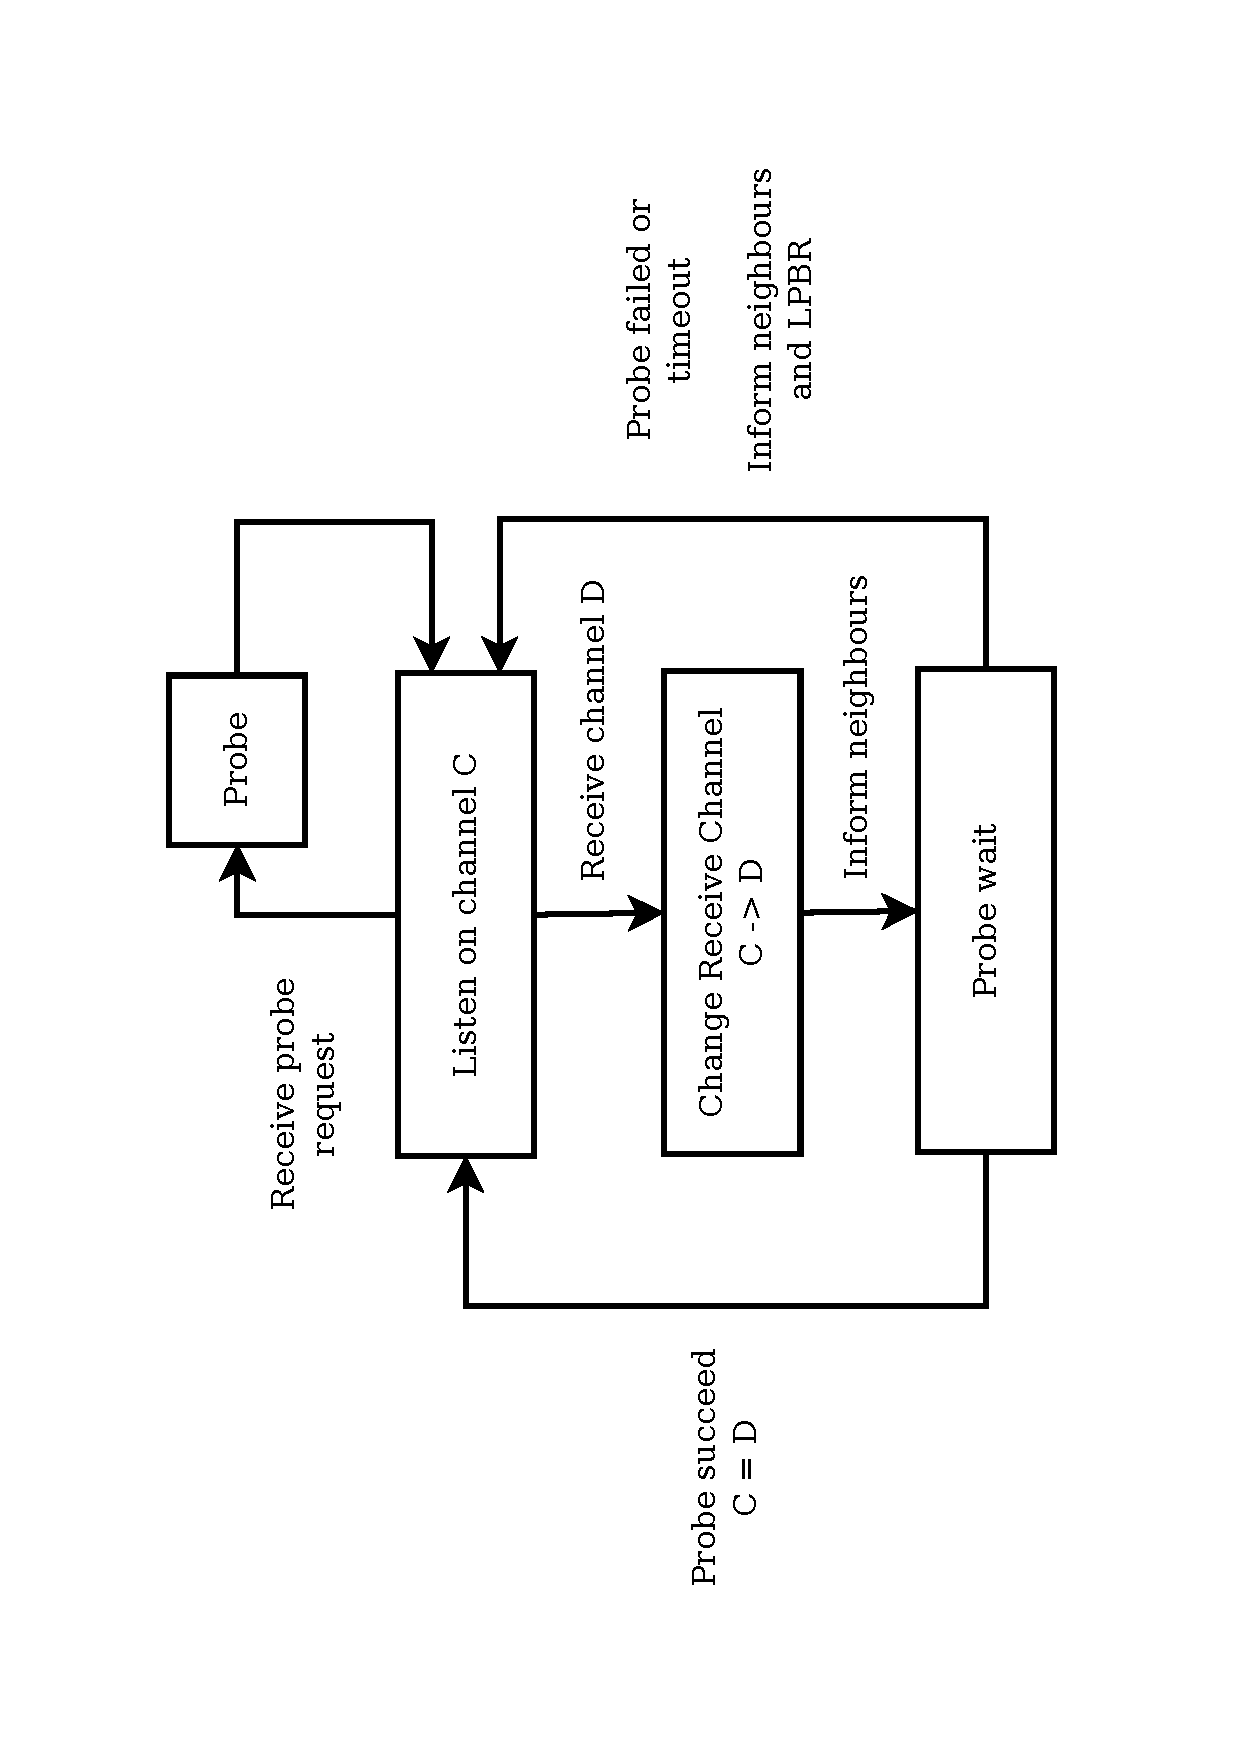
\includegraphics[trim=2cm 2cm 2cm 2cm, clip=true, totalheight=0.36\textheight, angle=270]{figures/channelSwitching.pdf}
%\caption{MCRP processes}
%\label{fig_mcrpDiagram}
%\end{figure}

Before a channel change MCRP uses probe packets between node $N$ and its neighbours to determine if the quality of channel is improved.  For each neighbour in turn eight probe packets are sent to $N$ on its new listening channel.  The number of packets received and the number of retransmissions required to receive them are monitored (in RPL several retransmissions are automatically tried).  The probing process fails if more than sixteen total transmissions are taken to receive eight packets on any link or if a timeout is reached before eight packets are received. In this case the node reverts to its previous channel.  The LPBR is informed of the results with a summary of all probes received and the channel so that the LPBR can build up a picture of channel strengths.

Because of the multichannel nature of MCRP a change is required to the RPL reconnection strategy to allow nodes that disconnect from their neighbour to find a new neighbour to connect to.  RPL uses a single channel and hence reconnection involves sending a message on this channel.  In MCRP these reconnection messages must be sent on multiple channels in turn as nodes are now listening on different channels.  New nodes and nodes which fall off the network can now rejoin on many potential channels.

\section{Energy-based Tree Reconfiguration}
\label{OptimalTree}

The expected number of transmissions (ETX) is calculated by nodes in RPL.  In MCRP nodes are selected to minimise this and channels are changed to minimise interference. However this does not account for the remaining battery life of nodes.  To do this MCRP is extended to reconfigure tree partners to maximise network lifetime.  

\subsection{Details of Tree Reconfiguration}

The next step in the process is to rearrange the tree to maximise network lifetime.  In this paper we take the definition that network lifetime is the time from the network set up until the first node failure.  Therefore, maximising network lifetime can be considered to be the problem of maximising the minimum predicted node lifetime over all nodes.  We alter the topology to achieve this since node lifetime is a function of the number of messages it sends.  However arbitrary topology rearrangement is not possible since firstly only some nodes are within communication range of others and secondly it would cause huge communication problems to make such a huge change.  Instead we consider ``swaps" where one node changes its parent to another node. The set of potential swaps is not large since not every node can see every other node.  Hence each node only has a small number of possible parents.  

It can be trivially shown that any topology can be reached by a series of swaps where a single node changes its parent node (since a topology can be completely defined in terms of the parent node for each node this takes at most $n$ swaps where $n$ is the number of nodes with a different parent in the target topology).  It is useful to define the ``children" of a node $i$ as those which have node $i$ as their parent and the ``descendents" of node $i$ as all thoses nodes that are below $i$ in the tree -- that is the children of $i$, the children of those children and so on.  It should also be noted that swapping nodes in the tree that are not $i$ or descendents of $i$ can not reduce the power consumption of node $i$ (since the number of messages going through $i$ cannot be reduced).  So only swaps to $i$ or its descendents need be considered.

 %(a) swap the parent of node $i$, (b) swap the children of node $i$, and (c) swap the descendants of node $i$ that are not the children. However, swapping the parent of the minimum lifetime node does not improve the node lifetime as the number of children and descendants remain same. Thus, only option (b) and (c) are further investigated.  

We next need an estimate of node lifetime.  Let $l_i$ be the current estimated lifetime of node $i$ (in arbitrary units).  This will be a function of the current energy and the number of messages it must send and receive.  Let $e_i$ represent the amount of energy remaining in the node (as a percentage of the total energy).  Let $d_i$ be the number of descendants, $t_{ij}$ represents the number of transmissions on average required to send a message from node $i$ to node $j$ (the ETX).  Let $p(i)$ be the node which is parent of $i$ and $c(i)$ be the set of children.  
We make the simplifying assumption that each node generates messages destined for the LPBR at the same average rate and since this rate constant $R$ would appear in all equations it may be dropped.  Node $i$ will receive $d_i$ messages from its descendents and generate 1 message itself. These messages require $t_{ip(i)}$ retransmissions giving $(d_i + 1)t_{ip(i)}$ messages and retransmissions to send them to the parent.  Each $j$ in the child set $c(i)$ will similarly wish to send $d_j + 1$ messages to $i$ and these messages are repeated $t_{ji}$ times on average.  Assuming sending and receiving messages gives an equal drain on battery life we therefore have
\begin{equation}
l_i = \frac{e_i}{{(d_i + 1)t_{ip(i)} + \sum_{j \in c(i)} (d_j + 1)t_{ji}}},
\label{optimalEq}
\end{equation}
no normalising constant is needed for the rate $R$ and for the cost of receiving/sending a message since $l_i$ is in arbitrary units.  If receiving a message has a different cost than sending a message then a normalising constant can be introduced before the sum.

A greedy algorithm is used to work out which swaps should be made in order.  This algorithm works as follows:
\begin{enumerate}
\item Calculate $l_i$ for all nodes.
\item Find $i$ such that $l_i$ is minimal.  The node $i$ is the node that will run out of energy first and $l_i$ is the current network lifetime estimate.
\item Create a set of possible swaps $S$ consisting of 
\begin{enumerate}
\item Swaps that move a non-child descendent of $i$ to be a direct child of $i$ (which may reduce the cost of messages to $i$ if that node now has reduced ETX).
\item Swaps that move a descendent of $i$ (including direct children) so that it is no longer a descendent of $i$ (which will reduce the number of messages through $i$.
\item Swaps that move a child of $i$ to be a non-child descendent of $i$ (if the new route has reduced ETX).
\item Swaps that move the parent of $i$ so that $i$ has reduced ETX to its parent.
\end{enumerate}
\item From the set $S$ calculate the swap that most improves network lifetime estimate.
\item If this new network lifetime is equal or larger to the current network lifetime estimate terminate the algorithm
\item Swap to the new topology and go to step 1).
\end{enumerate}

This algorithm greedily chooses topologies that improve lifetime at each step until no more swaps are available that will improve the network lifetime.

%\begin{algorithm}
%\caption{Pseudo-code for MCRP optimal tree algorithm}
%\label{mcrp_algo}
%\begin{algorithmic}[]
%\\\textbf{Notations}
%%\\$e_i$ is the node battery power
%\\$l_i$ is the node lifetime
%\\$c_i$ is the number of node $i$ children
%\\$d_i$ is the number of node $i$ descendants
%\\\textbf{Pseudo-code}
%\\Form tree based on MCRP
%\\Update battery level for all nodes
%\\Update all nodes $l_i$, $c_i$, $d_i$
%\\minimum $\leftarrow$ 0
%\\previousSwapNode $\leftarrow$ 0 
  %\While{node $\neq$ previousSwapNode}
    %\State Find node with minimum $l_i$
    %\State List all potential $c_i$ and $d_i$ swap
	%\If{$c_i$ and $d_i$ swap $l_i$ $>$ minimum} %to avoid cycle
		%\State Recalculate all nodes $l_i$
		%\If{all new nodes $l_i$ $>$ minimum}
			%\State Update tree
			%\State New tree is optimal
		%\Else
			%\State Revert to previous optimal tree
		%\EndIf
			%\State previousSwapNode $\leftarrow$ node
	%\Else
		%\State Current tree is optimal
	%\EndIf
  %\EndWhile
%\end{algorithmic}
%\end{algorithm}

%Algorithm \ref{mcrp_algo} describes the swapping processes based on the nodes lifetime calculated from Equation \ref{optimalEq}. It considers all available paths between the nodes and shows all potential topologies before deciding on the optimal tree.
%It is assumed that all nodes residual energy and the paths are known. Both the nodes battery and the link conditions can deteriorate over time. However, it is assumed that the current selected paths are the favourable routes selected by the MCRP, thus, only the battery level of the nodes is the variable. The topology is changed accordingly where the nodes that have the minimum value is selected to balance the network in term of the battery, link conditions and the number of children and descendants. The network is considered as balanced in term of the lifetime which means, the number of nodes and descendants connected might not be fairly distributed as the battery level vary in each node.

%\subsection{Illustrative Example}

%Figure \ref{fig:ot} is an illustrative example to explain the algorithm proposed. Assumed that the tree formed in Figure \ref{fig:ot-1} is the current optimal tree after running MCRP processes. Each node is labelled with the battery level, represented in percentage for simplicity. It can also be represented in volts or Joules. The lines between the nodes represent routes in different channels where dotted lines are the potential routes and the solid lines are the current routes. The values represent the link conditions in terms of the number of successful expected transmission between the two nodes. The values of the links are the expected transmission taken only for the upwards route as the links downwards could have different values due to the different transmission and reception channels on each node thus different link quality. 
%The transmission and reception channels of a node cannot be the same to avoid interference with nearby nodes.

%The figure shows that node 2 has the most descendants which consequently reduce the node lifetime as it has to forward more packets than any other nodes. Initially, the topology is formed based on the least value on the paths. In order to optimise the tree, the overall network lifetime is considered where paths that are not the minimum could be chosen as the route as it prolongs the overall functionality of the network. In this example, node 2 has the minimum lifetime. It can be maximised through swaps. 

%There are several potential swaps to improve node 2 lifetime that includes both the children which are node 5 and 6, and the children of children, node 7 and 8. Figure \ref{fig:ot-2} shows node 5 swaps to node 4 instead of its initial node 2 and the network lifetime is calculated. Node 2 lifetime is improved, however, node 1 has a lower lifetime than the initial minimum value as the result of swapping. Node 1 now has 5 descendants while node 2 only has one when it initially had 4. In order to reduce the number of unnecessary swap, once the maximum minimum lifetime is found, all nodes lifetime values are checked to ensure that they have higher lifetime than the initial minimum lifetime regardless of the maximising the minimum node to avoid endless cycle of swaps. While the swap done by node 5 improves node 2 lifetime, node 1 lifetime deteriorates to a value lower than the minimum. The network reverts to the previous topology that is better than the new swap. Node 5 tries and swaps to node 6, then node 6 swaps to node 8. However, the potential topology is not improved. Node 2 then swaps its descendants node 7 and 8.

%When node 7 is swaps to node 4 instead of node 5, the tree is improved. It can be seen in Figure \ref{fig:ot-3} that the tree is more balanced and node 2 lifetime is prolonged. As the result of swapping, node 4 lifetime is reduced as the path from node 7 to node 4 is not the smallest path value. The tree is updated as the current optimal tree. It is not yet the final optimal tree because node 8, which is another node 2 descendant has not been checked. If node 8 swap does not improve the tree, the swap from node 7 is chosen as the final optimal tree. 
%Another potential swap is shown in Figure \ref{fig:ot-4} where node 8 is connected to node 6 instead of node 5. In both cases, node 2 lifetime is maximised and all nodes lifetime are above the minimum value. The tree in Figure \ref{fig:ot-3} is selected as the final optimal tree in maximising node 2 lifetime. Further investigations are required in order to decide the criteria on an optimal tree when there are several good topologies to be selected. 

%Node 1 is then selected as the minimum lifetime as node 2 cannot be selected again to avoid unnecessary repetition. Optimal tree from the potential swaps for node 1 is not found thus the tree is said to be optimal. In the algorithm, the same node cannot swap again right after its previous swap. This is done to avoid oscillation which would produce similar result. The node however, could swaps in the next round as the other node swap would have changed the topology.

%The swaps are assumed to happen once until the network stops functioning, thus the overheads are negligible. The swapping calculations and decisions are made by the LPBR due to sensors limitations and constraints. LPBR informs the specific nodes of the final swapping if it needs to take place. In term of energy cost, the cost is negligible as the swaps are infrequent and being controlled by the LPBR.

%\begin{figure}
%\centering
%\subfigure[Initial tree]{\label{fig:ot-1}\includegraphics[page=1, trim=2cm 9cm 2cm 2cm, clip=true, totalheight=0.19\textheight]
%{figures/ot1.pdf}}        
%%\hfill        
%\subfigure[Node 5 swaps to node 4]{\label{fig:ot-2}\includegraphics[page=2, trim=2cm 9cm 2cm 2cm, clip=true, totalheight=0.19\textheight]
%{figures/ot1.pdf}}
%%\hfill        
%\subfigure[Node 7 swaps to node 4]{\label{fig:ot-3}\includegraphics[page=3, trim=2cm 9cm 2cm 2cm, clip=true, totalheight=0.19\textheight]
%{figures/ot1.pdf}}
%%\hfill        
%\subfigure[Node 8 swaps to node 6]{\label{fig:ot-4}\includegraphics[page=4, trim=2cm 9cm 2cm 2cm, clip=true, totalheight=0.19\textheight]
%{figures/ot1.pdf}}
%\caption{Graph of the bidirectional paths in a WSN}
%\label{fig:ot}
%\end{figure}

\section{MCRP Emulation Results}
\label{MCRPemulation}

MCRP is evaluated in the Cooja network emulator.  
Fifteen nodes are emulated for the communications network one LPBR and fourteen forming the tree of sensors.  In addition sixteen emulated nodes are used for interference.  
%TODO how are the nodes distributed.
Interference is generated using the model in~\cite{interferenceModel} using settings based on measurements in~\cite{radio2009}. The model has a clear state and an interfered state.  The rules for transitions between states are given in~\cite{interferenceModel}.  Here we allow four states according to the percentage of time where interfering signals are present: no interference, mild (75\% of the time no interference happens), moderate (50\% no interference) and extreme (25\% of the time no interference happens).  However, channel 26 is kept clear from interference in order to ensure RPL set up is unaffected. 

%In the interference state, the interference node generates packets for a time that is uniformly distributed between $9/16$ seconds and $15/16$ seconds. In the clear state the interferer produces no packets and stays in this state for between $3/4 * \emph{clear\textunderscore time}$ and $5/4 * \emph{clear\textunderscore time}$ where \emph{clear\textunderscore time} refers to the rate of interference (ir). 
%Multiple channels interference is used in the simulation to show the hypothesis that MCRP can help avoid interference. The scenario that is considered is where ContikiMAC with RPL system is subject to interference on its channel after set up has successfully completed so the RPL set up is allowed to complete before interference begins.

%The protocol performance in loss over time in the presence of interference is observed. The level of interference used in term of the \textit{clear\_time} is 100\% for no interference, 75\% for mild, 50\% for moderate and 25\% for extreme interference. The percentage represents the ratio of the time the channel is clear for transmission.
%The interference channels are randomly chosen from the available 16 channels.

The emulation has the following phases:
\begin{enumerate}
\item 0-5 minutes -- set up phase with no interference (this prevents RPL failing to build an initial tree in high interference situations).
\item 5-30 minutes -- interference nodes are switched on.  The MCRP tree building and reconfiguration begins.
\item 30-60 minutes -- interference continues and nodes attempt to send data every 30--60 seconds.  The rate of successful transmission is measured.
\end{enumerate}
Measurement of losses in the tree building phase is not made since this phase would be an unrepresentative one off set up cost for any protocol.  It is performance in the steady state that is important since this should last for weeks or years rather than tens of minutes.

The performance of MCRP is compared against the standard ContikiMAC with RPL and Orchestra to demonstrates MCRP abilities in dealing with external and intra interferences. 
%Orchestra does not support RPL downwards routing due to limited memory in TelosB. It however, support the upwards traffic which is require in the experiments as all traffics are directed upwards towards the LPBR.
MCRP is analysed using an end-to-end packet delivery performance metric, setup overhead, channel switching and reconnection delay in MCRP. The transmission success rate is calculated from the sender to the receiver over multiple hops. 
The simulations are repeated ten times. In all plots, the mean value of the ten simulations is plotted with error bars corresponding to one standard deviation in either deviation to give a measure of repeatability. The plots are of the proportion of received packets (from 0\% to 100\%) against time where the loss is measured over the previous time period.  The x-value is shifted slightly left and right to prevent error bars overlapping.

\subsection{Packet Loss Rates}

%\begin{figure}
%\centering
%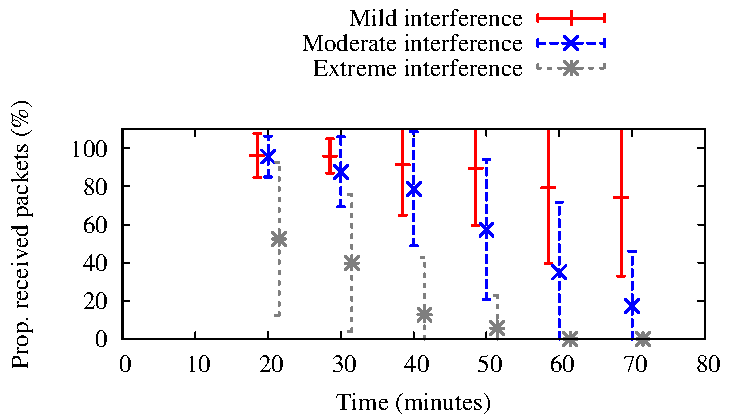
\includegraphics[width=0.45\textwidth]{figures/single_channel.pdf}
%\caption{Emulation: Level of packet loss for mild, moderate and extreme interference levels using single channel}
%\label{fig:interference}
%\end{figure}

%Figure \ref{fig:interference} shows the results in emulation for the single channel RPL protocol. This can be taken as a baseline for improvement for any multi-channel system.  It can be seen that as the emulation proceeds the proportion of received packets falls off.  The network 

Packet loss emulation results for interference on a single channel RPL system can be found in~\cite{mcrp}. These show that when interference is introduced to single channel RPL then the packet loss rate climbs quickly.  In the extreme interference case packet loss had climbed to 100\% by the end of the emulated period. For moderate interference this was 90\%.  For mild interference the figure was only 20\% but the variance was high.  These should be kept in mind as the levels a multiple channel system should improve upon.

\begin{figure}
\centering
\subfigure[Fixed layout]
{\label{fig:randomInterference}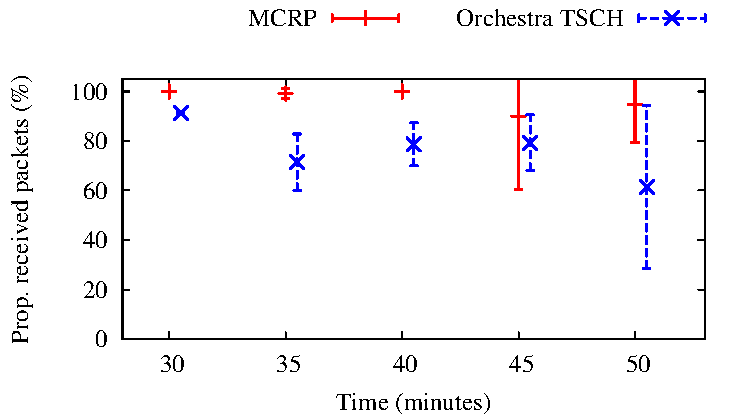
\includegraphics[width=0.45\textwidth]{figures/ri.pdf}}
\subfigure[Random layout]
{\label{fig:randomAll}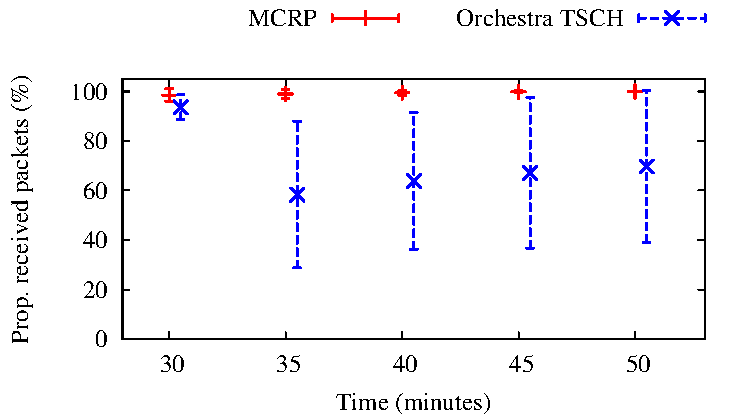
\includegraphics[width=0.45\textwidth]{figures/ra.pdf}}
\caption{Emulation: Level of packet loss for MCRP and Orchestra}
\label{fig:layouts}
\end{figure}


To evaluate MCRP capabilities to cope with interference from many sources, thus channels, and to compare to an existing multichannel protocol Orchestra, the emulations were run where (i) the layout is fixed while the interference channels are chosen by random and (ii) all the nodes including the interference nodes are placed randomly.
%in an area of $150m^2$.  In the fixed layout nodes were positioned in order that the fourteen nodes formed a tree where the LPBR has two children and each of those children has two children (four grand children) and each of those has two children (eight great grand children).
In the fixed layout nodes were positioned so that they formed a precise tree with the LPBR having two nodes directly attached and each of these child nodes having two nodes attached and each of these having two grandchild nodes. This produced a total of fifteen nodes including the LPBR. This was achieved by placing nodes that were to connect 10 metres apart. This distance was chosen so that nodes could form a good connection to the nodes next to them in the tree but nodes two hops away were too far to connect. In the random layout nodes were placed by choosing a uniformly random location within a square of side 150 metres.
In the experiments, Orchestra uses channel hopping on all 16 channels.  Interference is chosen randomly for the 16 channels so that 4 experience each of the interference conditions: no interference, mild interference, medium interfernce and extreme interference.


Figure \ref{fig:layouts} show MCRP and Orchestra results for the fixed and random nodes layouts.  In these graphs (and all graphs in this paper, x-axis values are shifted slightly to avoid error bars overlaying).
MCRP performs extremely well in both scenarios as the average packet reception rates are between 90\%-100\% and the protocol successfully detects the channels with interference.
Orchestra has higher packet loss compared to MCRP, showing a maximum of 40\% packet loss on average as the channels with interference are being used for transmission periodically. 
In comparison, MCRP selects certain channels to change into after checking the channels condition which gives MCRP a smaller number of packet loss.
MCRP avoids the interference channel while Orchestra hops to the next channel in the next iteration for transmission.

\subsection{Overheads of multiple channel protocols}

Changing channels and probing channels requires signalling overhead for set up.  Extra messages need to be passed for probing and to change channels.  Estimations for setup overhead are given in ~\cite{mcrp}.  Default RPL on ContikiMAC for the topology considered in these experiments completed its set up using 276 packets. MCRP, the multi-channel protocol completed its set up in 716 packets, that is an overhead of 440 packets on top of RPL.  However, it is worth mentioning that this is a one-off cost representing (in this set up) approximately one hour of extra packets where the sensor network deployment would be expected to be in place for weeks, months or longer.  The set up time is 1154 seconds longer for MCRP than RPL.

%Each node has different listening and transmitting channels. When the node is awake, it waits for incoming packets on its listening channel. If the node has a packet to send, it will switch to the next hop listening channel based on the channel information from the neighbour table. The channel switching takes at most 100$\mu$ to switch to the transmission channel. This delay is negligible in the low packet rate WSN. MCRP ContikiMAC uses a transmission phase-lock where the transmission node knows the receiver wake up phase. The node starts transmitting just before the receiver is expected to be awake. The channel switching happens shortly before the receiver is ready to receive the packets, thus the time taken in channel switching does not affect the packet reception.
%The node goes back to sleep once the transmission has succeeded or reached the maximum number of retransmissions (packet loss). In the next iteration, the node is reset and wakes up on its listening channel. 

%The channel reset is done in these cases: (i) the queue buffer is empty, (ii) before sending the next packet from the queue buffer, and (iii) the last packet in the queue buffer has been sent. This reset is done to avoid any delay in packet reception that could happen when the node is awake.2


MCRP also has overhead compared to RPL in terms of reconnection time.  MCRP nodes that disconnect must probe multiple channels to reconnect to the network (as described in section \ref{sec:switching}).  This is obviously slower than RPL that only need probe a single channel.  To test this in isolation we deliberately disconnected a network in the absence of interference by disabling a parent node and measuring the effect on packet transmission.

In the Figure~\ref{fig:reconnectionLayout} node 3 is disabled.
Node 6 and 7 route through node 3 to the LPBR. Nodes 6 and 7 must reconnect through node 5 as shown in Figure \ref{fig:r2}. 

\begin{figure}
\centering
\subfigure[Initial tree]{\label{fig:r1}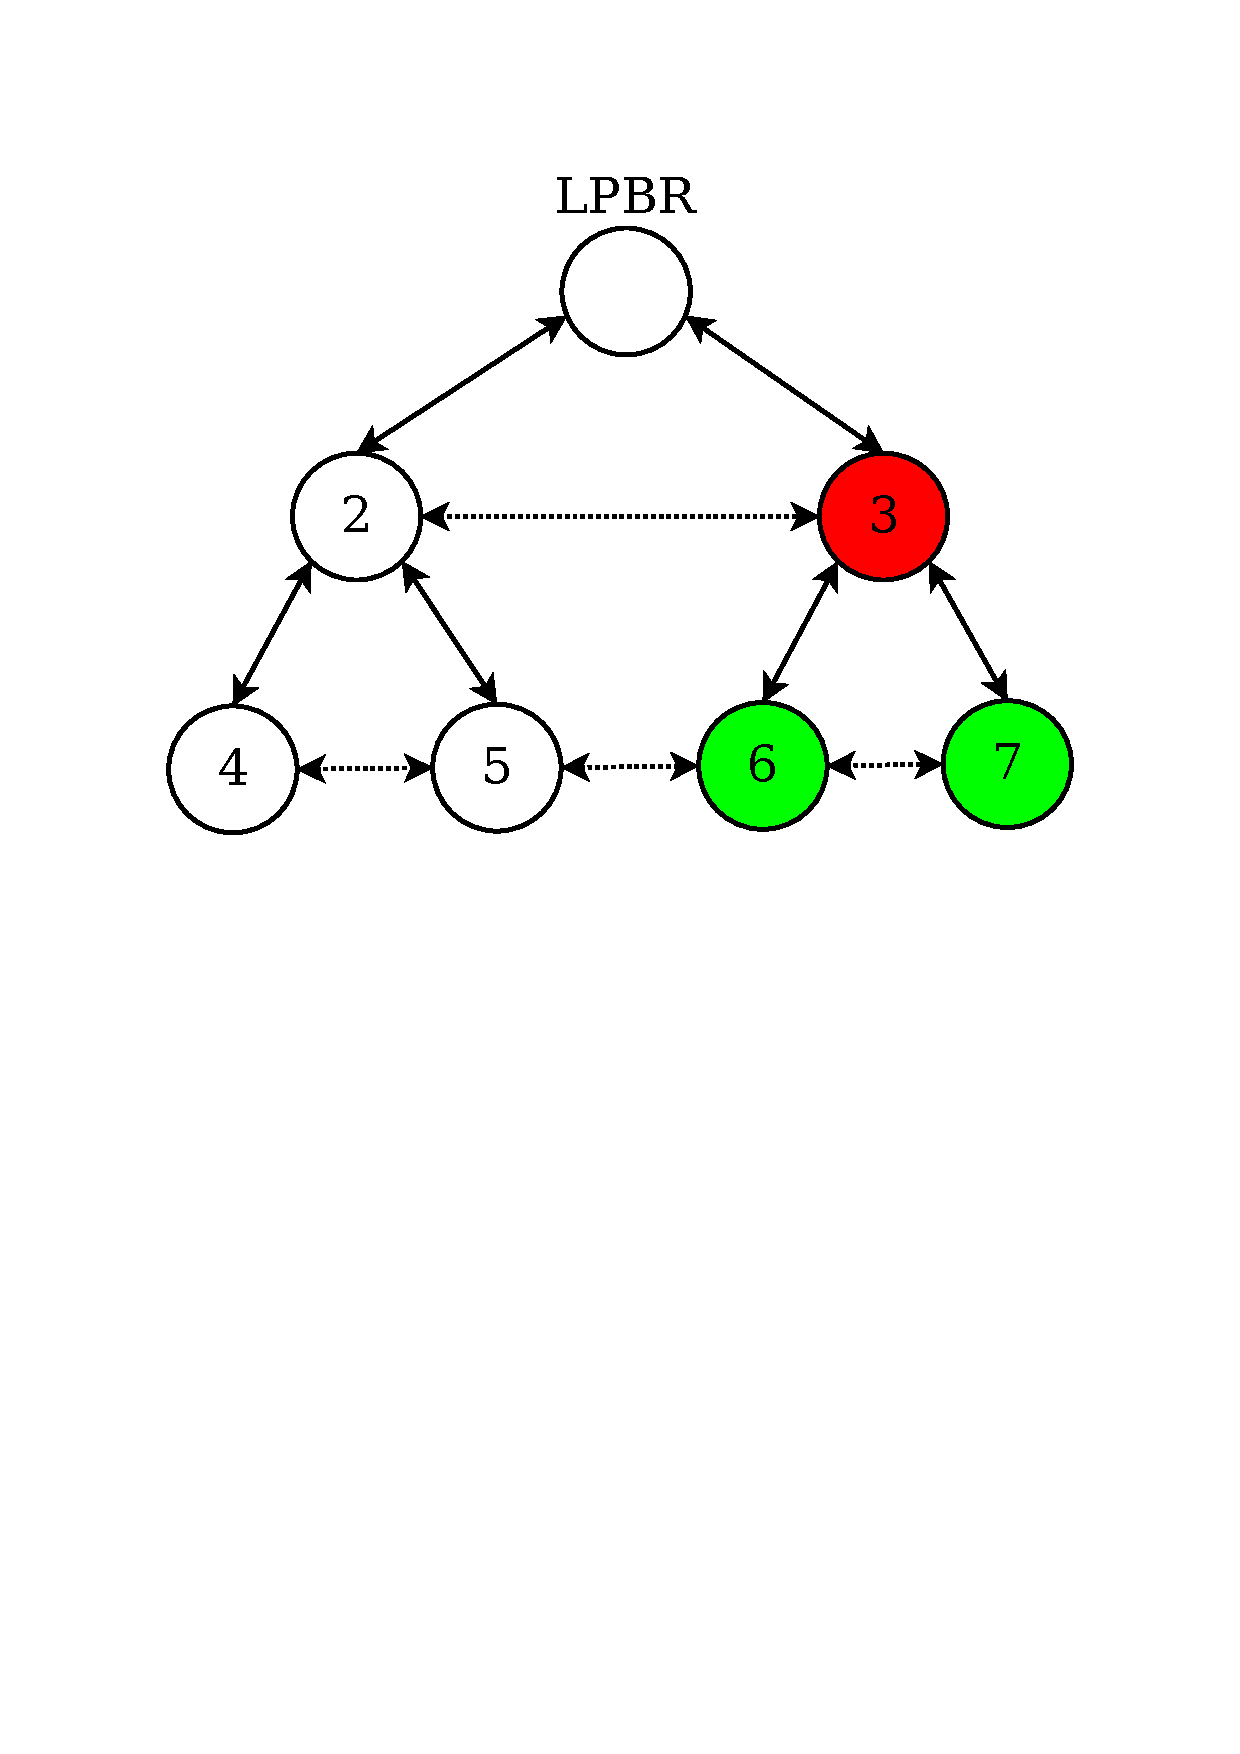
\includegraphics[trim=2cm 15cm 2cm 2cm, clip=true, totalheight=0.12\textheight]
{figures/reconnection1.pdf}}        
\hfill        
\subfigure[Reconstructed tree when node 3 is undetected]{\label{fig:r2}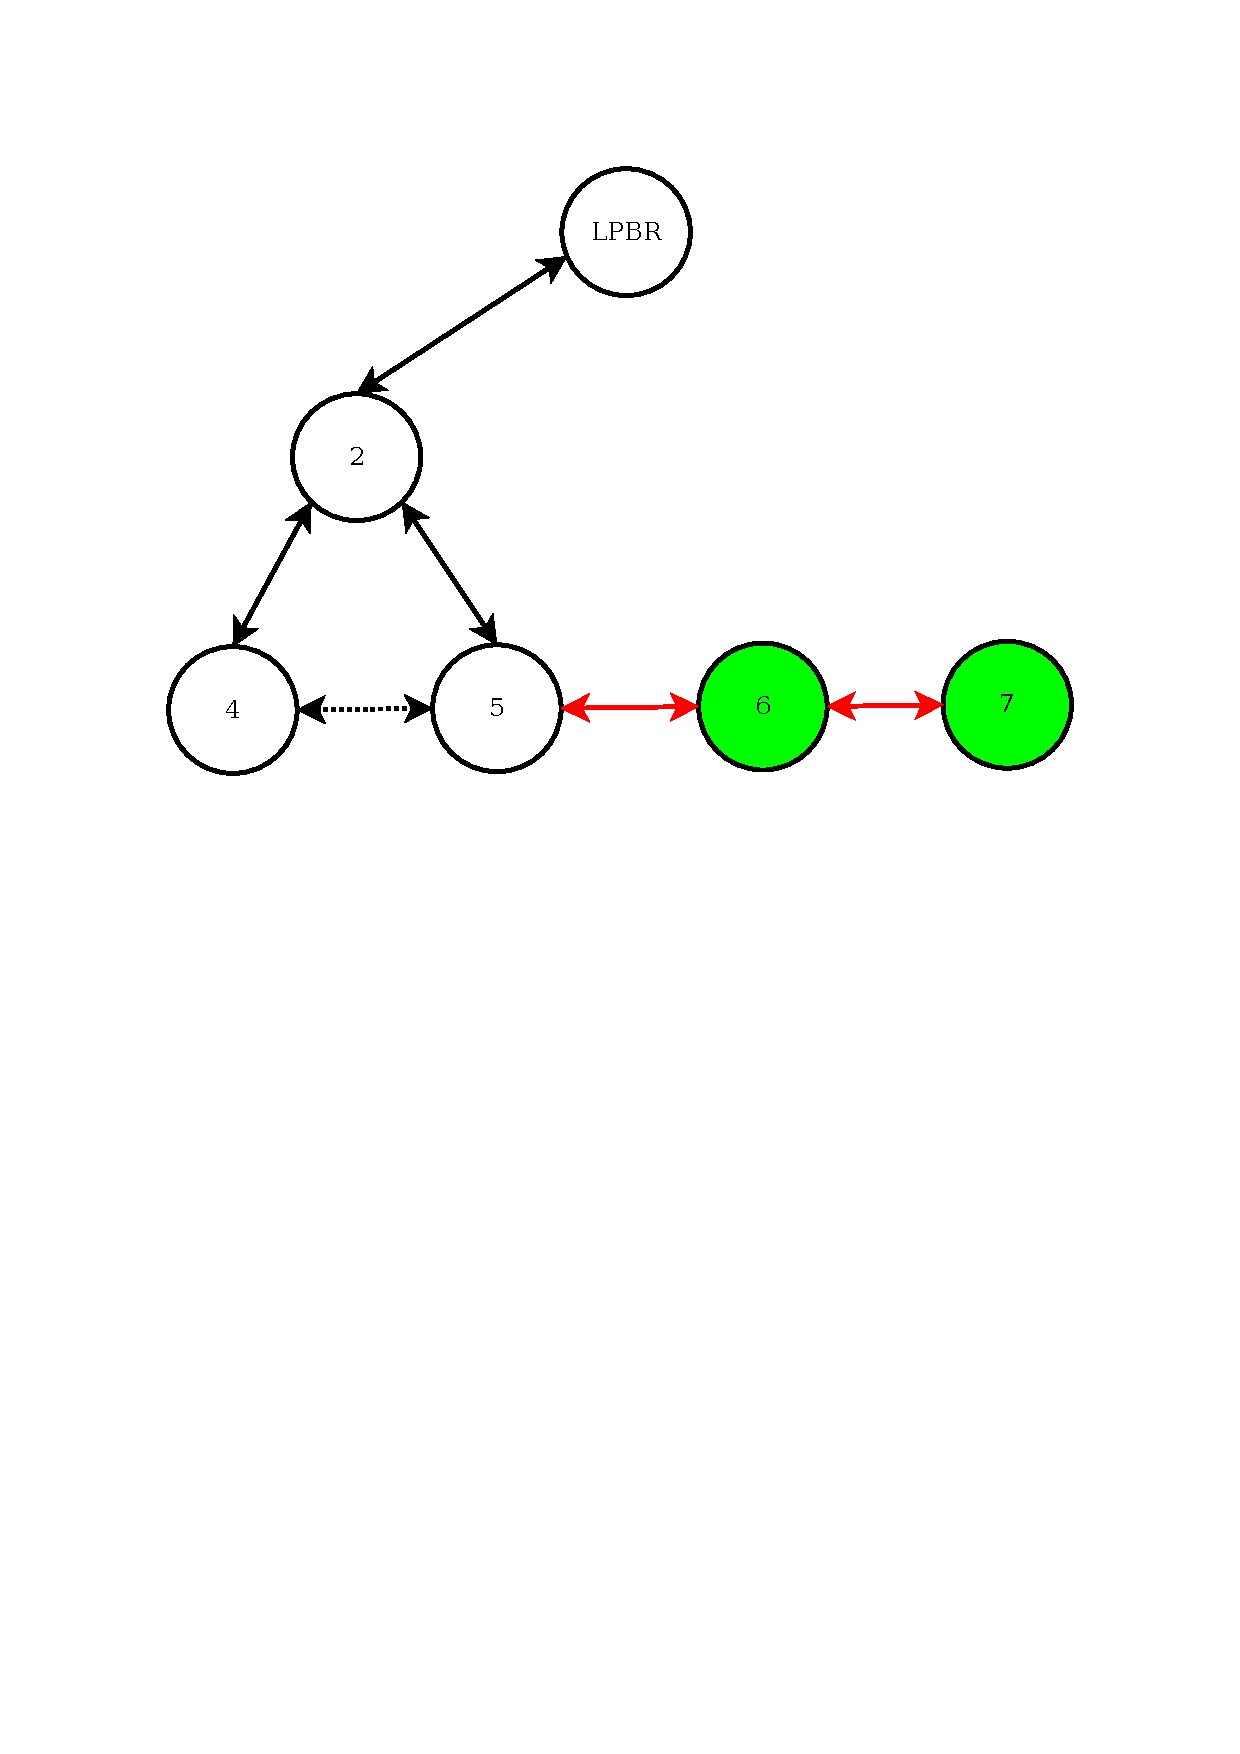
\includegraphics[trim=2cm 15cm 2cm 2cm, clip=true, totalheight=0.12\textheight]
{figures/reconnection2.pdf}}
\caption{A simple tree to emulate the tree reconnection}
\label{fig:reconnectionLayout}
\end{figure}

Figure \ref{fig:reconnection} shows the result of disconnecting node 3 after 54 minutes of emulation.  In MCRP, it took between five and seven minutes before nodes 6 and 7 reconnect.  RPL with single channel is slightly quicker taking three to five minutes. However, considering the more complex task MCRP is performing two minutes added onto reconnection time in the context of a network with low data rates should be acceptable considering the other performance advantages.  In the Orchestra system, by contrast, reconnection is almost instantaneous since the synchronous Orchestra system checks nodes every slot but this is at the expense of greatly increased control traffic.

\begin{figure}
\centering
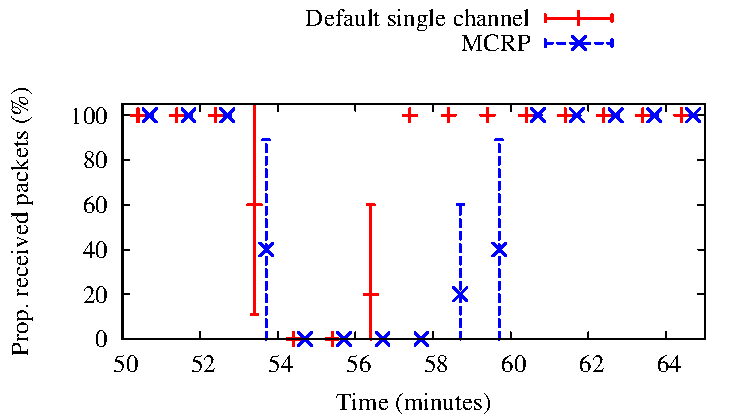
\includegraphics[width=0.45\textwidth]{figures/reconnect.pdf}
\caption{Emulation: Reconnection time taken for MCRP and single channel}
\label{fig:reconnection}
\end{figure}

%Figure \ref{fig:reconnectionLayout} shows the experimental setup to test MCRP reconnection in term of the time taken to detect and adjust the routes when a node fails (run out of battery or cannot be detected). There is no external interference introduced to ensure an accurate convergence time of the topology. The dotted lines represent potential paths and the solid lines are the selected paths. The result from MCRP is compared to a single case scenario with the same setup.


%Comparing to Orchestra, Orchestra is a synchronous protocol. It has a dedicated slot and periodic schedule for RPL signalling which means it detects the failed node quicker unlike in MCRP and default single channel asynchronous protocols. The results from the Orchestra simulation shows that as Orchestra has a slot checking the nodes every minute, it is able to reconnect the nodes without having any packet loss. The disadvantages of Orchestra are, the nodes are listening on the same channel during the broadcast which the known channel is prone to attack. Also, even though Orchestra introduces priority to the traffic, RPL traffic is sent frequently at every period if there is no other higher priority traffic. Trickle timer that is used by the default RPL has the advantage of reducing the number of redundant control packets by doubling the waiting time for the control packets. Orchestra detects failed node quicker at the cost of frequent control packets that are redundant in a stable topology which increases the use of bandwidth and nodes energy consumption.

\subsection{MCRP Hardware Performance Evaluation}
\label{MCRPhardware}

Experiments are also implemented on hardware in realistic environments.  The hardware is tested in both home and office environments since~\cite{homearea} suggests that the two are drastically different.  The same experimental set up is tried in each environment.  The test network consists of 10 nodes; 1 border router and 9 duty cycled nodes.  At the highest power level nodes have a range of approximately 25 metres.  In indoor experiments this would mean that most nodes were in direct communication.  To change this we set the power level to -40dB relative to maximum giving a range of 15-80 cm (depending on intervening interference).  At this power level not all nodes are in direct communication but the positions were selected to allow each node to be in range of at least one other in order that a tree forms.  For the single channel protocol experiment each channel is measured for interference.  The protocol is tested on the channel with the lowest interference and the channel with the highest interference.

The first section of the experiment is "warm up" to allow for network formation.  This is forty five minutes for MCRP to complete set up and channel changes. During the experiment period four hundred and fifty packets are sent in total, fifty from each node at a rate of one per minute.  Each experiment is repeated ten times.  End-to-end packet delivery is used as the performance metric.  Unlike in the emulation results, the RPL tree formation set up is affected by the interference during initialisation. The network could be formed differently at each iteration.  

Nodes with direct connection to the LPBR must send on the LPBR listening channel and hence do not benefit from multi-channel.  However, several nodes were able to run MCRP processes. The tree topology formed differently each time depending on the radio coverage and interference level which affect the RPL ETX value for next hop selection. By increasing the number of nodes and area coverage, it increases the chances that the nodes would have routes to or from which enables MCRP to be executed.  

\begin{figure}
\centering
\subfigure[Residential environment]
{\label{fig:hardwareHome}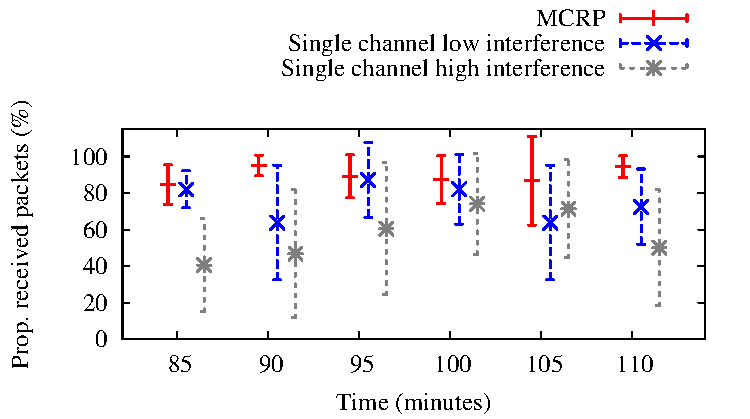
\includegraphics[width=0.45\textwidth]{figures/home.pdf}}
\subfigure[Office environment (UCL)]
{\label{fig:hardwareUCL}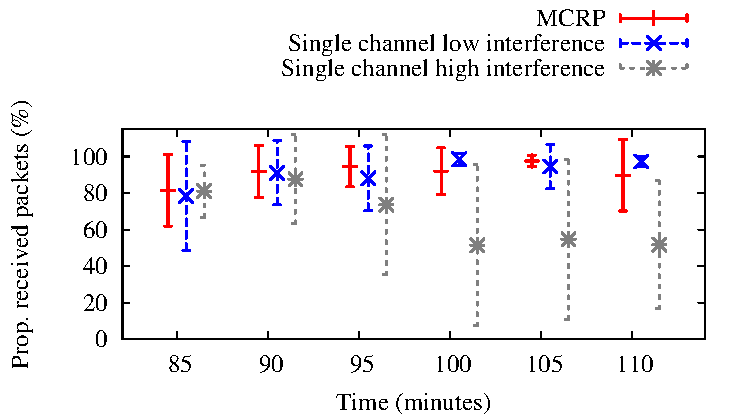
\includegraphics[width=0.45\textwidth]{figures/ucl.pdf}}
\caption{Real world: Level of packet loss for MCRP and single channel}
\label{fig:hardware}
\end{figure}

Figure \ref{fig:hardware} show the results from the experiment in residential and office environments for MCRP compared to the single channel protocol results for the channel with lowest interference and the channel with highest interference.  It can be clearly seen that in all experiments the error bars are high indicating that performance is extremely variable between runs of the experiment.  The MCRP protocol had higher mean packets received than the single channel protocol with high interference and comparable mean with the single channel protocol with low interference.  The MCRP protocol tended to have lower variance in performance particularly in the residential environment.  This demonstration shows that MCRP works on real hardware in realistic settings.  There was little demonstrated performance gain, possibly because of the small number of nodes used but MCRP did have more consistent performance in terms of packets received.

%% This file is not used
\subsection{Energy Improvement from MCRP}

Multichannel protocol not only could reduce the end to end delay, it also helps to improve the nodes energy efficiency by ensuring minimal packet retransmissions thus energy consumption.
MCRP implements Contiki's existing energy module, Powertrace.
Powertrace uses the software based on-line energy estimation mechanism \cite{dunkels2007software} to estimate the node's current energy consumption in real time. 
The energy estimation module uses time measurements that can be directly obtained from the microprocessor on-chip timer when the component is switched on to produce a time stamp. The time difference from when the component was on and when it later is switched off is computed. The current draw of the component listed in the TelosB data sheet is used to compute the total energy consumption estimation, $E$. 

\begin{equation}
E = (I_{m}t_{m} + I_{l}t_{l} + I_{tx}t_{tx} + I_{r}t_{r} +  \sum_{i}I_{c_{i}}t_{c_{i}}) \times{V}
\label{energyModel}
\end{equation}

Equation \ref{energyModel} shows the energy consumption model given in \cite{dunkels2007software}  
where $V$ is the supply voltage, $I$ is the current draw and $t$ is the active time computed in Powertrace for $m$ the microprocessor, $l$ the microprocessor in low power mode, $tx$ the communication device in transmit mode, $r$ the communication device in receive mode and $c_{i}$ for other components such as sensors and LEDs. The values of $I_{m}$, $I_{l}$, $I_{tx}$ and $I_{r}$ are device dependent. 

Powertrace is used to compute the energy consumption estimation of the network. However, the nodes do not have enough capability to compute their individual energy consumption. In order to estimate the energy taken from the sender to the receiver, each node sends their energy values to LPBR regularly as MCRP has a centralised controller. This enables LPBR to predict the energy drain if the routes have high interference or packet losses. LPBR is able to compute the end to end energy consumption on each routes and estimate the nodes battery level based on the energy values. Each node sends the energy value of its packet transmission, packet forwarding and total time value that the radio has been on from the beginning to LPBR for energy consumption computation.
By doing that, the nodes knowledge of its energy level is kept at minimum. 

In order to calculate accurate energy consumption for specific packet transmission, the unicast packet type is separated into normal unicast and control messages unicast. The unicast packet from the application layer (normal unicast) is set as \textit{unicastMsg = 1}, which the value is 0 by default to represents other unicast packets. This allows the energy of the transmission packet to be calculated separately without including other control messages that could be sent right after or before the normal packet transmission. This is done to avoid inaccurate energy spent as control messages are only being sent periodically unlike the normal packet that are sent frequently. It also enables retransmit packets to be included as the current transmission packet energy. This will alert the LPBR on the current condition of the node with much higher energy consumption than the usual energy per packet because of the retransmissions. The $unicastMsg$ value is reset when the link layer acknowledgement is received or the maximum number of retransmission is reached. 

\subsection{Energy Performance Evaluation}
 
The energy consumption in MCRP in term of transmission per packet, forwarding packets energy and total energy used are computed to prove that multichannel helps to prolong the network lifetime by using the energy more efficiently than in a single channel network. Each node sends one packet per minute, 350 packets in total throughout the simulation period. Equation \ref{energyModel} is used to calculate the nodes energy consumption. The energy consumption of each node is computed by the LPBR based on the information contained in the transmitted packet. The maximum number of hops in the simulation is 3 hops. The results of a single channel with no interference is used as the base case as it is the ideal energy consumption value. The results are also compared to the energy of a single channel with moderate and extreme interference, and MCRP for multi channels.

\subsubsection{Energy Per Packet Performance}

\begin{figure}
\centering
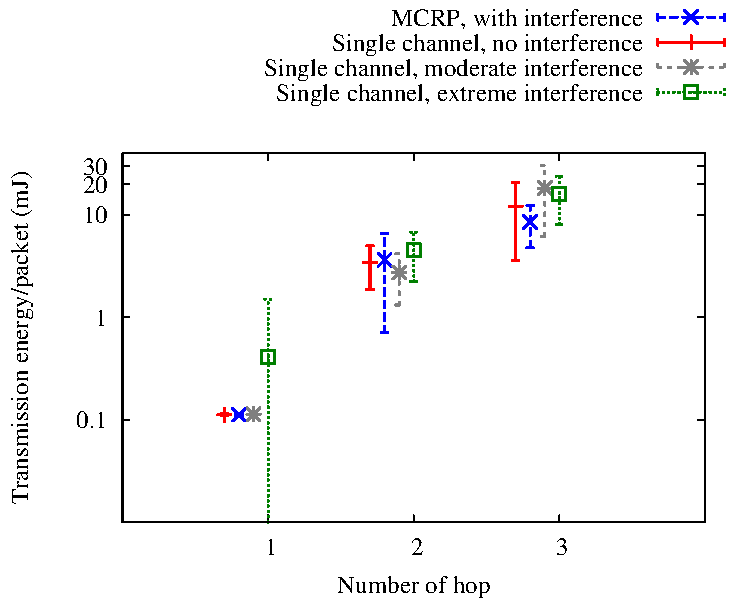
\includegraphics[width=0.45\textwidth]{figures/perPktEnergy.pdf}
\caption{Simulation: The energy consumption per packet in different number of hops}
\label{fig:energyPerPkt}
\end{figure}

Figure \ref{fig:energyPerPkt} shows the transmission energy per packet for nodes that are 1, 2 and 3 hops away from the LPBRs. From the figure, it can be concluded that less transmission energy is used when there is less number of hops. However, in a large scale network, the number of hops cannot be reduced as not all nodes would be in the range or directly connected to the destination node. Thus, the node's next hop should be selected carefully to avoid nodes that have higher interference rate.

In the 1 hop case, it can be seen that the nodes consumed approximately similar energy in all cases. As the nodes are one hop to the destination (LPBR), it was not affected by the interference except for a slight variation in the single channel with extreme interference case. 
Nodes that are 2 and 3 hops away show higher values of per packet energy transmission.
This is because of the interference near to the nodes. The nodes are unable to detect the exact wake-up time for the nodes thus, the nodes have to transmit in a longer period to ensure the packet gets transmitted. In the one hop graph, the energy can be kept at minimum because the LPBR is always awake to accept packet as it is fully powered unlike the other nodes that have to switch the radio off when there are no transmissions and receptions taking place to save the energy.

In the 1 and 2 hops, MCRP shows approximately similar transmission energy consumption to the base case. 
In 3 hops, the energy per packet in the single channel with moderate and extreme interference are much higher than the energy used by the base case and MCRP. This shows that the energy per packet depends on the number of hops and the interference that affect the routes. Multichannel helps to mitigate the effect of interference, thus reducing the transmission energy taken to send a packet especially when there are several hops involved.

\subsubsection{Total Energy Consumption}

\begin{figure}
\centering
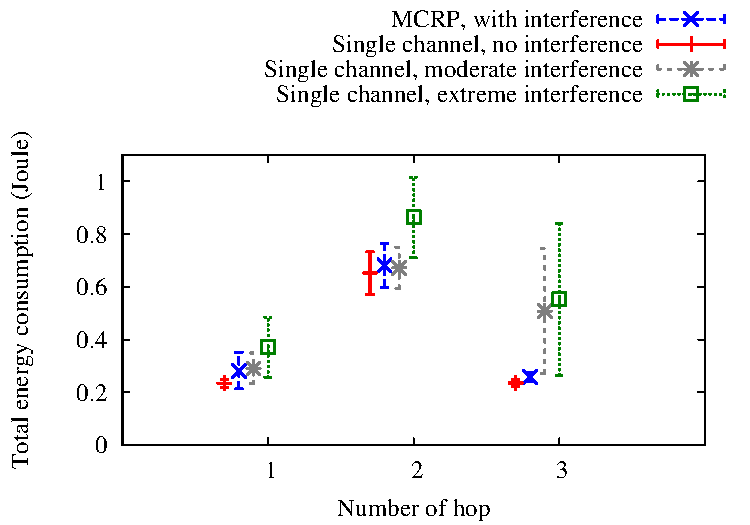
\includegraphics[width=0.45\textwidth]{figures/totalEnergy.pdf}
\caption{Simulation: The nodes total energy consumption}
\label{fig:allNodesEnergy}
\end{figure}

Figure \ref{fig:allNodesEnergy} shows the total energy consumption in the simulation including retransmissions and control packets energy.  
In 1 hop, it can be seen that in all cases, the total energy taken are approximately similar with a small standard deviation. The single channel with extreme interference case however, requires higher energy consumption than in other cases.
In 2 hops, it shows high increase in energy usage. The reason for this is because the 2 hops nodes are used as forwarding nodes. The 3 hops nodes do not act as forwarding nodes thus the reason for the lower total energy consumption.
The energy consumption is improved when using MCRP than a single channel with interference. This improvement can be clearly seen in the 3 hops nodes where MCRP uses 3 times less energy than in the single channel cases of an approximate 0.6 Joules as these nodes use more energy during interference for retransmissions. If the retransmissions fail, the packet is dropped and the energy used during the retransmissions is wasted. The total energy consumption graph shows all energy spent when the nodes are awake, including forwarding and failed packets transmission.

\subsubsection{Forwarding Energy Analysis}

\begin{figure}
\centering
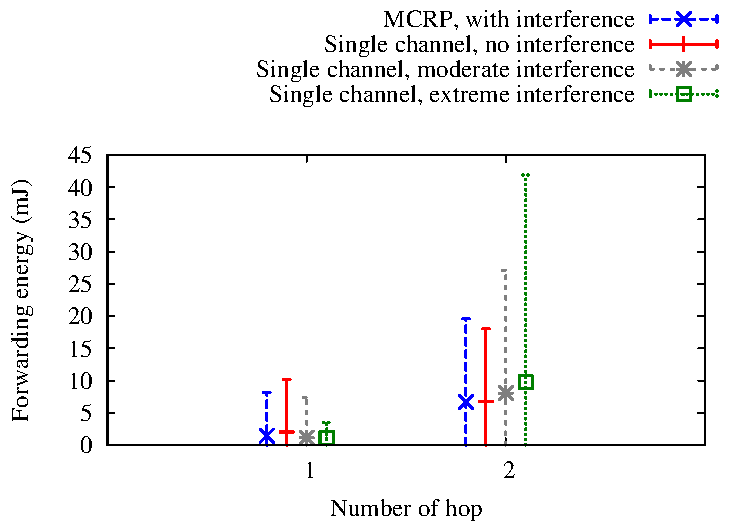
\includegraphics[width=0.45\textwidth]{figures/fwdEnergy.pdf}
\caption{Simulation: The nodes forwarding energy}
\label{fig:allNodesFwdEnergy}
\end{figure}

Figure \ref{fig:allNodesFwdEnergy} shows the energy used in forwarding packets for the 1 and 2 hops nodes. The 3 hops nodes in the simulation do not forward packets. The 1 hop nodes use less energy than the 2 hops nodes as the nodes only need to check if the channel is being use by the other node before it can forward to the LPBR. LPBR waits for incoming packet thus the nodes could send the packet with less waiting time as LPBR radio is always on. 
In order to be able to forward the packets, the nodes have to be awake for longer time and ensure the intermediate node is also awake and ready to accept the packets. Thus forwarding could require more energy consumption than an end to end packet transmission. By increasing the number of nodes thus children, the nodes will use more energy in order to forward the packets. The forwarding energy consumption contributes to the most energy used by the nodes.  
Even though MCRP does not show a lot of improvement, it shows lower deviation compared to the single channel with extreme interference.
In the base case, the energy consumption varies as the nodes are interfering with each other even without external interference during transmissions.

The simulation results showed that MCRP consumes less energy than in other cases when there is interference as the effect of multichannel. MCRP has similar energy consumption values as in the base case, a single channel without interference. This shows that multichannel helps to reduce the energy wasted due to interference. In order to increase the energy efficiency thus network lifetime, MCRP needs to reconstruct the topology based on the energy consumption, residual energy of the nodes and the link conditions gradually to avoid breaking any current connectivity.

\section{Network lifetime evaluation}
\label{PerformanceEvaluation}

This section describes the evaluation of the network lifetime extension algorithm.  We measure (a) the average number of switches to form the improved tree and (b) the impact of swapping on the network lifetime.  As mentioned in section \ref{OptimalTree} we define the network lifetime as the time until first node failure, that is the smallest value of $l_i$ from (\ref{optimalEq}).  Because lifetimes must be evaluated over extremely long periods with large numbers of nodes, simulation is used instead of emulation.

\subsection{Simulation Setup}

The improved tree algorithm from section \ref{OptimalTree} is simulated in the C programming language. The number of sensors considered is varied between 10 to 500 and each node is randomly assigned an initial energy between 50\% to 100\%. The link conditions are also randomly assigned the value between 1 to 10 indicating the ETX (1 being a clear channel with no retransmission and 10 meaning ten retransmissions on average). In this setup, the channels are fixed, assuming that the current channels that the nodes are listening and transmitting on, are the best selected channels from the previous MCRP processes. RPL builds the initial tree based on the ETX value which is then further improved by MCRP. In order to avoid all the nodes from directly connecting to the LPBR, each node could route to a minimum of $1/10$ and $1/30$ of the total number of nodes.
This allows the node to have alternative parents (thus paths) for the swapping processes and hops to reach the LPBR. The node is not necessarily connected to all $1/10$ and $1/30$ nodes. The paths between the nodes are selected based on the RPL and MCRP processes. These values are selected in the case where (a) the nodes are closely together ($1/10$), and (b) the nodes are spread out with minimum connections to the other nodes available ($1/30$). 

\subsection{Simulation Results}
\subsubsection{Average Number of Switches}

\begin{figure}
\centering
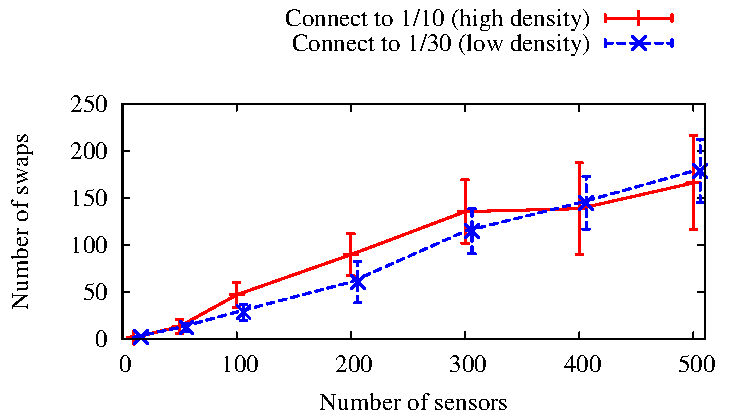
\includegraphics[width=0.45\textwidth]{figures/swaps.pdf}
\caption{Simulation: Average number of swaps}
\label{fig:aveSwaps}
\end{figure}

Figure \ref{fig:aveSwaps} shows the standard deviation and average number of swaps using MCRP improved tree algorithm. 
It can be observed that there are more swaps on average when there are more sensors in the network in both connection cases. However, nodes that could route to $1/10$ of the total sensors showed slightly higher number of swaps than in the $1/30$ connection. The reason for this is because in $1/10$ connection, it has more neighbours, hence many potential parents to select. 

In a smaller network, the sensors are limited by the number of potential parents. This prevents the nodes from swapping as the potential parents might not have any improvement. This can be seen from the number of swaps in a 50 sensors network where the average number of swaps is less than 10. This is because each node has 5 (in $1/10$) and 2 (in $1/30$) potential parents to select from unlike in the 500 sensors network which each has 50 and 17 potential parents. However, as there are more sensors, it takes longer to find the best parents as the swaps will consider all nodes that are within the range.

This experiment does not reflect the condition in the real world where the sensors could be scattered with more or less available range to the other nodes depending on the application; which means more nodes can directly be connected to the LPBR without hops in between. This however, represents a reasonable connection between the nodes to allow swapping and alternative nodes if the current forwarding nodes values are at a minimum for the experiment.


\subsubsection{Impact On The Network Lifetime}

\begin{figure}
\centering              
\subfigure[Connect to 1/10 of total sensors]{\label{fig:1-10}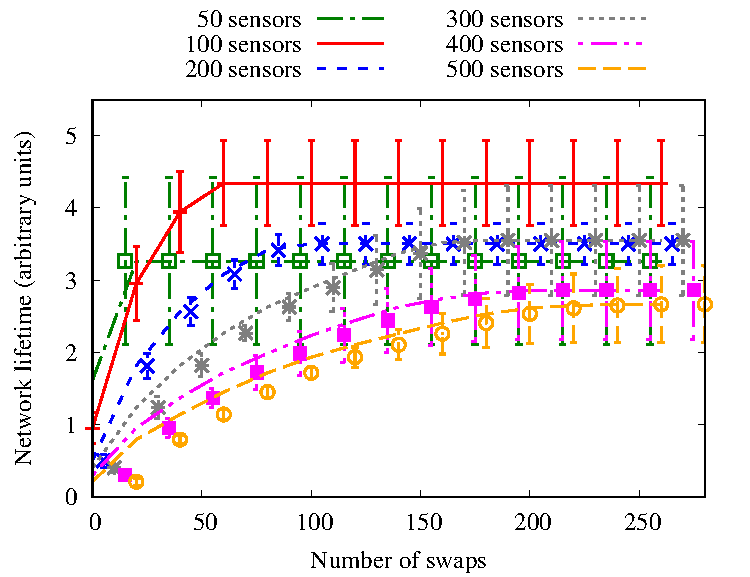
\includegraphics[width=0.45\textwidth]{figures/lifetime1.pdf}}
\subfigure[Connect to 1/30 of total sensors]{\label{fig:1-30}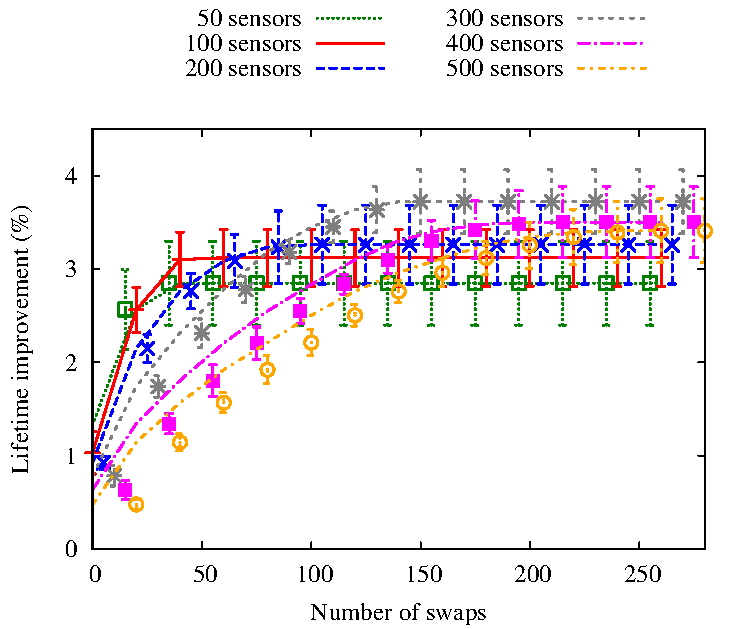
\includegraphics[width=0.45\textwidth]{figures/lifetime3.pdf}}
\caption{Simulation: Comparison of the number of swaps and lifetime in different network scale}
\label{fig:maxmin}
\end{figure}

Figure \ref{fig:maxmin} shows the improvement in the node thus network lifetime by maximising the minimum and the number of swaps required in 10 runs in 6 networks with 50, 100, 200, 300, 400 and 500 sensors with different degree of connection. 
The standard deviation on the x axis is slightly shifted to prevent the error bars from overlapping.
It is observed that the node lifetime decreases with an increase in the number of sensors in the network. The reason for this is in a larger network, there are a higher number of descendants and each connection has its own path values. By taking into account these variables, the number of nodes affect the whole network lifetime. While a higher number of nodes allow more alternative routes, it also consumes more energy as there are more connected nodes. Smaller network however, has limited number of possible swaps which does not improve the network lifetime.

Figure \ref{fig:1-10} shows the number of swaps and the lifetime when the nodes are connected to $1/10$ of the total nodes in the network. 
In the 50 nodes network, the number of swaps is less than 10 before it reaches the maximum lifetime for the whole network. 
As the number of sensors in the network increase, it takes more swaps before the tree is improved. 
In the 200 nodes network, the number of swaps is around 100 swaps and the lifetime is improved by a factor of 7, an increase from 0.5 to 3.5. In 500 nodes network, it takes more swaps, around 200 swaps for the lifetime is improved by a factor of 9, an increase from 0.3 to 2.7.

Figure \ref{fig:1-30} shows similar improvement in the $1/30$ connection case. However, it can be seen that the maximum lifetime values in the figure for 100 sensors network is slightly less than in Figure \ref{fig:1-10}. This is because the networks have lesser potential parents and paths to select from. The tree is limited by the number of connections. The other large networks have similar maximum lifetime values in both figures.

\begin{figure}
\centering
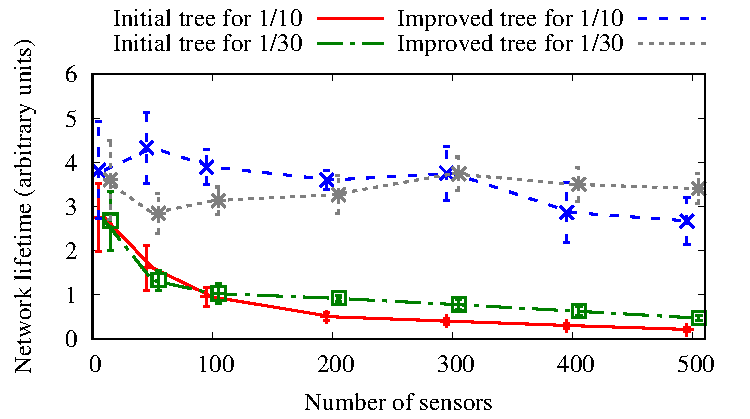
\includegraphics[width=0.45\textwidth]{figures/maxmin.pdf}
\caption{Simulation: Lifetime of MCRP improved tree}
\label{fig:nodes-maxmin}
\end{figure}

Figure \ref{fig:nodes-maxmin} shows the comparison between the initial and improved tree in both cases. MCRP swapping prolongs the network lifetime which shows an increase from the initial lifetime. Smaller networks have high initial lifetime values compared to larger networks.  This is because in large networks there are always a few nodes that have to carry a great amount of traffic.  However, larger networks have better lifetime improvement than the slight improvement in smaller networks.

In the initial trees, it can be seen that when there are more sensors in the network, the lifetime values are decreasing. This shows the importance of finding the improved tree as the results showed that the lifetime can be improved by a factor of 9 in the 500 nodes network.
%four times. 
The increase enables the network to remain functional slightly longer than initially. 


\section{Conclusion}
\label{Conclusion}

This paper introduced Multichannel Routing protocol (MCRP) which consists of a protocol for multi-channel use of Wireless Sensor Networks and an algorithm for channel selection. The paper also introduced a topology changing procedure that greedily changes the topology of a WSN to improve the estimated network lifetime.  MCRP was tested in hardware for small networks, in emulation for larger networks and in simulation for networks with several hundred nodes.  MCRP shows high packet reception rate of nearly 100\% of the ideal (zero interference) rate in simulations and 80\%-90\% in real-world tests on hardware. In addition, MCRP reduces the energy consumption at an average node by a factor of 3 due to the multichannel system avoiding interference.  The energy-based tree reconfiguration is proposed to further improve the multichannel network by considering the energy level of each sensor and forming a topology that places less load on nodes with low power. 
This enables the network to be fully functional for a longer period of time and extends sensor lifetime.  The system showed an increase in the network lifetime increasing the time until first node failure by a factor of 8.3 (over a static topology) in a simulated 500 node system.


% use section* for acknowledgment
%\section*{Acknowledgment}
%The authors would like to thank...

\label{references}
%\nocite{*}
\bibliography{main}
\bibliographystyle{IEEEtran}

%\subsection{Subsection Heading Here}
%Subsection text here.

%\subsubsection{Subsubsection Heading Here}
%Subsubsection text here.


% An example of a floating figure using the graphicx package.
% Note that \label must occur AFTER (or within) \caption.
% For figures, \caption should occur after the \includegraphics.
% Note that IEEEtran v1.7 and later has special internal code that
% is designed to preserve the operation of \label within \caption
% even when the captionsoff option is in effect. However, because
% of issues like this, it may be the safest practice to put all your
% \label just after \caption rather than within \caption{}.
%
% Reminder: the "draftcls" or "draftclsnofoot", not "draft", class
% option should be used if it is desired that the figures are to be
% displayed while in draft mode.
%
%\begin{figure}[!t]
%\centering
%\includegraphics[width=2.5in]{myfigure}
% where an .eps filename suffix will be assumed under latex, 
% and a .pdf suffix will be assumed for pdflatex; or what has been declared
% via \DeclareGraphicsExtensions.
%\caption{Simulation results for the network.}
%\label{fig_sim}
%\end{figure}

% Note that the IEEE typically puts floats only at the top, even when this
% results in a large percentage of a column being occupied by floats.


% An example of a double column floating figure using two subfigures.
% (The subfig.sty package must be loaded for this to work.)
% The subfigure \label commands are set within each subfloat command,
% and the \label for the overall figure must come after \caption.
% \hfil is used as a separator to get equal spacing.
% Watch out that the combined width of all the subfigures on a 
% line do not exceed the text width or a line break will occur.
%
%\begin{figure*}[!t]
%\centering
%\subfloat[Case I]{\includegraphics[width=2.5in]{box}%
%\label{fig_first_case}}
%\hfil
%\subfloat[Case II]{\includegraphics[width=2.5in]{box}%
%\label{fig_second_case}}
%\caption{Simulation results for the network.}
%\label{fig_sim}
%\end{figure*}
%
% Note that often IEEE papers with subfigures do not employ subfigure
% captions (using the optional argument to \subfloat[]), but instead will
% reference/describe all of them (a), (b), etc., within the main caption.
% Be aware that for subfig.sty to generate the (a), (b), etc., subfigure
% labels, the optional argument to \subfloat must be present. If a
% subcaption is not desired, just leave its contents blank,
% e.g., \subfloat[].


% An example of a floating table. Note that, for IEEE style tables, the
% \caption command should come BEFORE the table and, given that table
% captions serve much like titles, are usually capitalized except for words
% such as a, an, and, as, at, but, by, for, in, nor, of, on, or, the, to
% and up, which are usually not capitalized unless they are the first or
% last word of the caption. Table text will default to \footnotesize as
% the IEEE normally uses this smaller font for tables.
% The \label must come after \caption as always.
%
%\begin{table}[!t]
%% increase table row spacing, adjust to taste
%\renewcommand{\arraystretch}{1.3}
% if using array.sty, it might be a good idea to tweak the value of
% \extrarowheight as needed to properly center the text within the cells
%\caption{An Example of a Table}
%\label{table_example}
%\centering
%% Some packages, such as MDW tools, offer better commands for making tables
%% than the plain LaTeX2e tabular which is used here.
%\begin{tabular}{|c||c|}
%\hline
%One & Two\\
%\hline
%Three & Four\\
%\hline
%\end{tabular}
%\end{table}


% Note that the IEEE does not put floats in the very first column
% - or typically anywhere on the first page for that matter. Also,
% in-text middle ("here") positioning is typically not used, but it
% is allowed and encouraged for Computer Society conferences (but
% not Computer Society journals). Most IEEE journals/conferences use
% top floats exclusively. 
% Note that, LaTeX2e, unlike IEEE journals/conferences, places
% footnotes above bottom floats. This can be corrected via the
% \fnbelowfloat command of the stfloats package.


%\appendices
%\section{Proof of the First Zonklar Equation}
%Appendix one text goes here.

% you can choose not to have a title for an appendix
% if you want by leaving the argument blank
%\section{}
%Appendix two text goes here.



% Can use something like this to put references on a page
% by themselves when using endfloat and the captionsoff option.
\ifCLASSOPTIONcaptionsoff
  \newpage
\fi



% trigger a \newpage just before the given reference
% number - used to balance the columns on the last page
% adjust value as needed - may need to be readjusted if
% the document is modified later
%\IEEEtriggeratref{8}
% The "triggered" command can be changed if desired:
%\IEEEtriggercmd{\enlargethispage{-5in}}

% references section

% can use a bibliography generated by BibTeX as a .bbl file
% BibTeX documentation can be easily obtained at:
% http://mirror.ctan.org/biblio/bibtex/contrib/doc/
% The IEEEtran BibTeX style support page is at:
% http://www.michaelshell.org/tex/ieeetran/bibtex/
%\bibliographystyle{IEEEtran}
% argument is your BibTeX string definitions and bibliography database(s)
%\bibliography{IEEEabrv,../bib/paper}
%
% <OR> manually copy in the resultant .bbl file
% set second argument of \begin to the number of references
% (used to reserve space for the reference number labels box)

%\begin{thebibliography}{1}

%\bibitem{IEEEhowto:kopka}
%H.~Kopka and P.~W. Daly, \emph{A Guide to \LaTeX}, 3rd~ed.\hskip 1em plus
%  0.5em minus 0.4em\relax Harlow, England: Addison-Wesley, 1999.

%\end{thebibliography}

% biography section
% 
% If you have an EPS/PDF photo (graphicx package needed) extra braces are
% needed around the contents of the optional argument to biography to prevent
% the LaTeX parser from getting confused when it sees the complicated
% \includegraphics command within an optional argument. (You could create
% your own custom macro containing the \includegraphics command to make things
% simpler here.)
%\begin{IEEEbiography}[{\includegraphics[width=1in,height=1.25in,clip,keepaspectratio]{mshell}}]{Michael Shell}
% or if you just want to reserve a space for a photo:

%\begin{IEEEbiography}{Noradila Nordin}
%Biography text here.
%\end{IEEEbiography}

%\begin{IEEEbiography}{Richard G Clegg}
%is a Lecturer in Networks at Queen Mary University of London. His PhD is in mathematics and statistics from the University of York was gained in 2005. His research interests include investigations of the dynamic behaviour of networks and measurement of network traffic statistics.
%\end{IEEEbiography}

%\begin{IEEEbiography}{Yiannis Andreopoulos}
%Biography text here.
%\end{IEEEbiography}

%\begin{IEEEbiography}{Miguel Rio}
%Biography text here.
%\end{IEEEbiography}

%% if you will not have a photo at all:
%\begin{IEEEbiographynophoto}{John Doe}
%Biography text here.
%\end{IEEEbiographynophoto}

% insert where needed to balance the two columns on the last page with
% biographies
%\newpage

%\begin{IEEEbiographynophoto}{Jane Doe}
%Biography text here.
%\end{IEEEbiographynophoto}

% You can push biographies down or up by placing
% a \vfill before or after them. The appropriate
% use of \vfill depends on what kind of text is
% on the last page and whether or not the columns
% are being equalized.

%\vfill

% Can be used to pull up biographies so that the bottom of the last one
% is flush with the other column.
%\enlargethispage{-5in}



% that's all folks
\end{document}


